\chapter{Super-Resolução de Imagens Pós-Inversão}
\label{cap:3modeloHibrido}

Neste Capítulo é apresentada a metodologia discutida neste trabalho.
São apresentadas as estratégias iniciais de aplicação do modelo convolucional,
os resultados preliminares obtidos e o cronograma de atividades.

\section{Modelo de Super-Resolução}

Este trabalho propõe desenvolver um modelo de rede neural convolucional para
realizar supre-resolução de imagens da inversão sísmica acústica.
No capítulo anterior foi apresentado o método de inversão acústica que
representa o estado da arte no cálculo do máximo \textit{a posteriori} (MAP) para determinar o
resultado mais provável \citep{Buland01012003, Figueiredo2014}. Foram apresentados os trabalhos relacionados
com o desenvolvimento de modelos de redes neurais convolucionais para tratar problemas de
super-resolução \citep{Oord16,He2016,DahlNS17}. 
% 
A presente proposta tem como objetivo o emprego de um modelo de rede neural convolucional
para aumentar a resolução das imagens de impedância acústica
resultantes do processo de inversão sísmica. Com esta abordagem se espera obter um ganho
quantitativo, através da inserção de altas frequências no espectro de frequência da
propriedade, e qualitativo, através de imagens com maior definição entre camadas.
Além disto, por se tratar de um problema de inversão, um estudo de incerteza sobre os
resultados das redes convolucionais será realizado sobre os resultados.

A proposta de adaptação e expansão do modelo apresentado por
\cite{DahlNS17} parece viável, pois apresenta os fundamentos para o desenvolvimento
de modelos convolucionais condicionados. Entretanto, o modelo apresentado por
\cite{} funciona como uma rede classificadora, de modo que os valores previsos
pela rede são discretos. Para ser aplicado sobre dados geoestatísticos o modelo
necessita ser ajustado. Esta mudança visa tornar o modelo capaz de realizar regressão
diretamente sobre os valores de impedância, ou para impedância normalizada no intervalo real
$[-1,+1]$.

A rede convolucional é um modelo cujo treinamento é supervisionado, de modo que,
para ajustar seus parâmetros, é necessário dispor dos pares de imagens de alta
resolução e a baixa resolução. Uma vez a rede convolucional treinada,
imagens de baixa resolução provenientes de outros cenários de inversão podem ser aplicadas ao modelo.

Para realizar a inversão acústica é necessário ter disponível a sísmica, a \textit{wavelet}
e o modelo de baixa frequência para impedância acústica ($<8Hz$) %(Equação \ref{eqn:mapSolution}).
O fluxo de trabalho segue as etapas listadas:
 
\begin{enumerate}
  \item Parametrização do método de inversão acústica com a sísmica, a \textit{wavelet} e o modelo de baixa frequência.
  \item Geração das imagens de baixa resolução
  \item Normalização das imagens de impedância para escala de cinza.
  \item Divisão do conjunto de dados entre conjunto de treinamento e conjunto de teste.
  \item Treinamento do modelo de rede convolucional com os pares de imagens de treinamento.
  \item Amostragem das imagens de alta resolução a partir das imagens de teste de baixa resolução.
  \item Comparação entre as imagens obtidas da rede e a imagem real.
  \item Recuperação dos valores de impedância das imagens de alta resolução obtidas.
\end{enumerate}

As questões a serem respondidas neste trabalho são: o modelo de rede convolucional é capaz de aumentar a Resolução de imagens de impedância
quantitativamente? As imagens de teste apresentaram maior resolução que as imagens originais, sob o ponto 
de vista de altas frequências? Quais as faixas de alta frequências foram inseridas? Como as redes neurais aprenderam
as altas frequências? É possível parametrizar o processo de super-resolução para imagens pós-inversão?
Qual o limite de alta frequência é possível inserir nas imagens de alta resolução? Existe coerência geoestatística
no resultado do modelo convolucional? Investigar a possibilidade de adaptação da rede para diferentes tipos de \textit{upscaling}.


\section{Resultados Preliminares}
Como experimento do modelo inicial foram usados dois conjuntos de dados sintéticos.


 
\subsection{Caso sintético: Cunha}

%Explicar a geração das imagens de cunha
%Deixar claro o uso de imagens 32 x 32 mostrar a região de teste apliada da imagem total
\subsection{Caso sintético: impedância Acústica}
Para realizar o segundo experimento foi utilizado um cubo sintético de impedância
acústica com 239 imagens de dimensões 250 x 199. Do cubo de impedância foram calculados os
valores de refletividade. Uma \textit{wavelet}
sintética foi estimada e o cubo sísmico foi obtido por meio da
convolução entre a refletividade e a \textit{wavelet}.
O cubo de impedância foi filtrado abaixo de $8Hz$ para obter o modelo de baixa frequência e
um ruído foi adicionado à sísmica.

Explicar o uso do método de Leandro para gerar as imagens:


-falar da parametrização.

Falar do conjunto de dados composto por pares de imagens de alta e baixa resolução:

\subsection{Transformada rápida de Fourier}
%Explicar a aplicação da transformada de Fourier como métrica de comparação entre as imagens

% 
% Experimentos realizados com o método para cálculo do MAP obtiveram resultados e
% tempo de execução comparáveis com métodos implementados na indústria
% \citep{leandroGRSL}. Apesar de resultar somente nas médias e variâncias, a
% parametrização e regularização utilizada na metodologia pode ajudar a restringir
% a amostragem, de forma a inserir informações da posterior e tornar a amostragem
% do SSD mais eficiente.
% 
% 
% Como a inversão GSI é fundamentada na Simulação Sequencial Direta, os resultados
% da primeira iteração da GSI são iguais aos resultados de uma SSD utilizando os
% mesmos parâmetros e dados de entrada. Desta forma é possível verificar a melhora
% na correlação da sísmica sintética com a sísmica original quando se utiliza o
% resultado do MAP como imagem secundária para SSD. Este experimento foi realizado
% e na primeira iteração do GSI a correlação das sísmicas sintética e original foi
% $0.45$ para a média de impedância, com a SSD utilizando o resultado do MAP como
% imagem secundária foi obtida uma correlação de $0.97$ para a média, foram
% utilizadas populações de $35$ amostras para cada método. Mesmo quando são
% executadas as iterações da GSI, a máxima correlação da média encontrada é $0.9$,
% tomando no mínimo 10 iterações para atingir este nível de qualidade.
% 
% Foram utilizados dados fornecidos pela PETROBRAS de um campo real para efetuar
% os testes. Os dados consistem de 4 poços que se encontram na posição dos traços
% 17, 210, 409 e 698, modelo de baixa frequência interpolado dos poços, horizontes
% e uma \textit{wavelet} extraída por um especialista da empresa. O parâmetro de
% distância de correlação da inversão por MAP foi utilizado $L=1.4$, a variância da sísmica
% foi estipulada como $0.4$ multiplicado pela variância média dos traços.
% Para a SSD foi utlizado um modelo de variograma horizontal omnidirecional
% esférico com alcance de $32$ traços, ou aproximadamente $800$ metros. Para o
% variograma vertical foi utilizando o mesmo modelo com o alcance de $2$ índices
% de tempo, correspondente a $8ms$.
% 
% O resultado da inversão MAP é demonstrado na Figura \ref{fig:mapResult}.
% A média das realizações amostradas pelo método proposto está na Figura
% \ref{fig:mapDSS}. Comparando com a Figura \ref{fig:dssresult}, a qual demonstra
% a média das realizações da primeira iteração da GSI, verifica-se que utilizar o
% resultado do MAP como imagem secundária traz a informação da sísmica nos pontos
% entre dos poços. Comparando a média da GSI após 10 iterações, na Figura
% \ref{fig:dss10result}, observa-se a semelhança dos resultados sem a necessidade
% de realizar as iterações. O método proposto demorou 52s para executar contra
% 487s para realizar as 10 iterações da GSI.
% 
% 
% 
% \begin{figure}[htp]
% \begin{center}
%   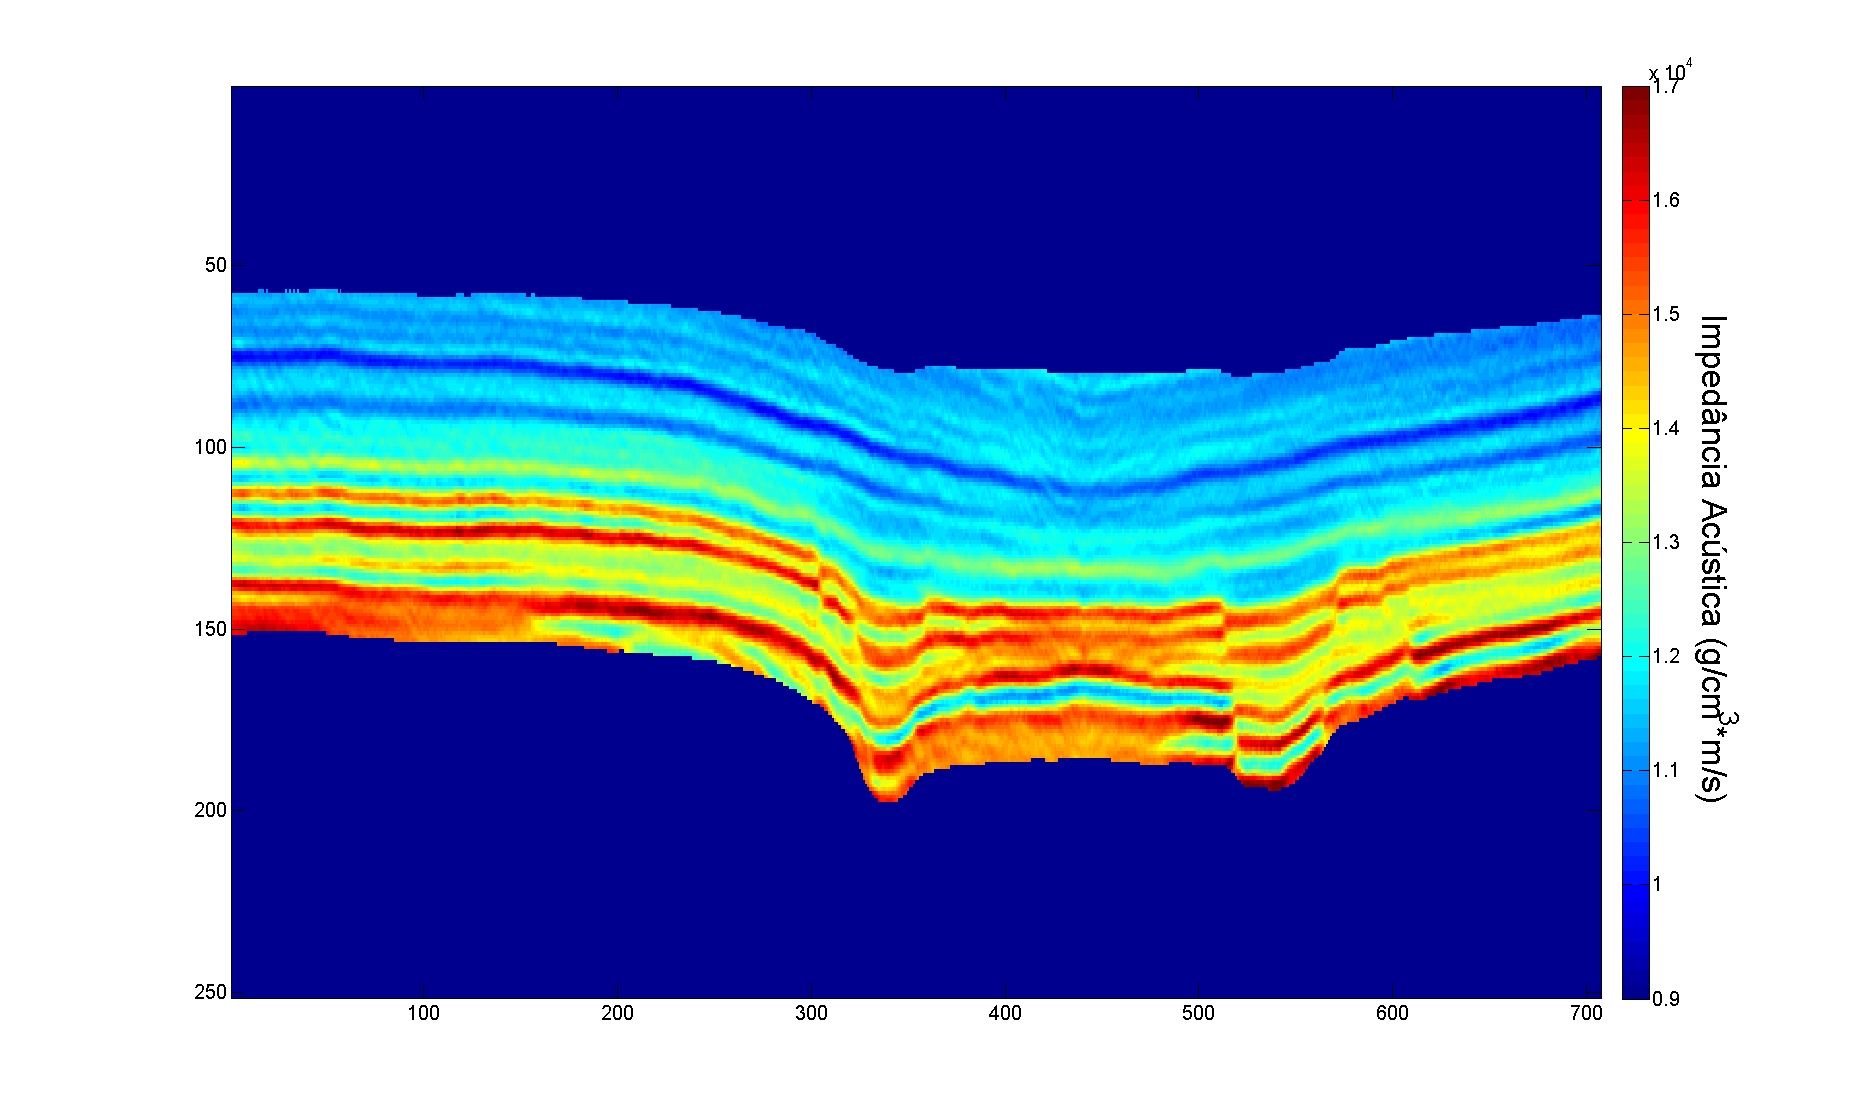
\includegraphics[width=\textwidth]{fig/map}
%   \caption{Resultado MAP utilizado como imagem secundária}
%   \label{fig:mapResult}
% \end{center}
% \end{figure}
% 
% 
% \begin{figure}[htp]
% \begin{center}
%   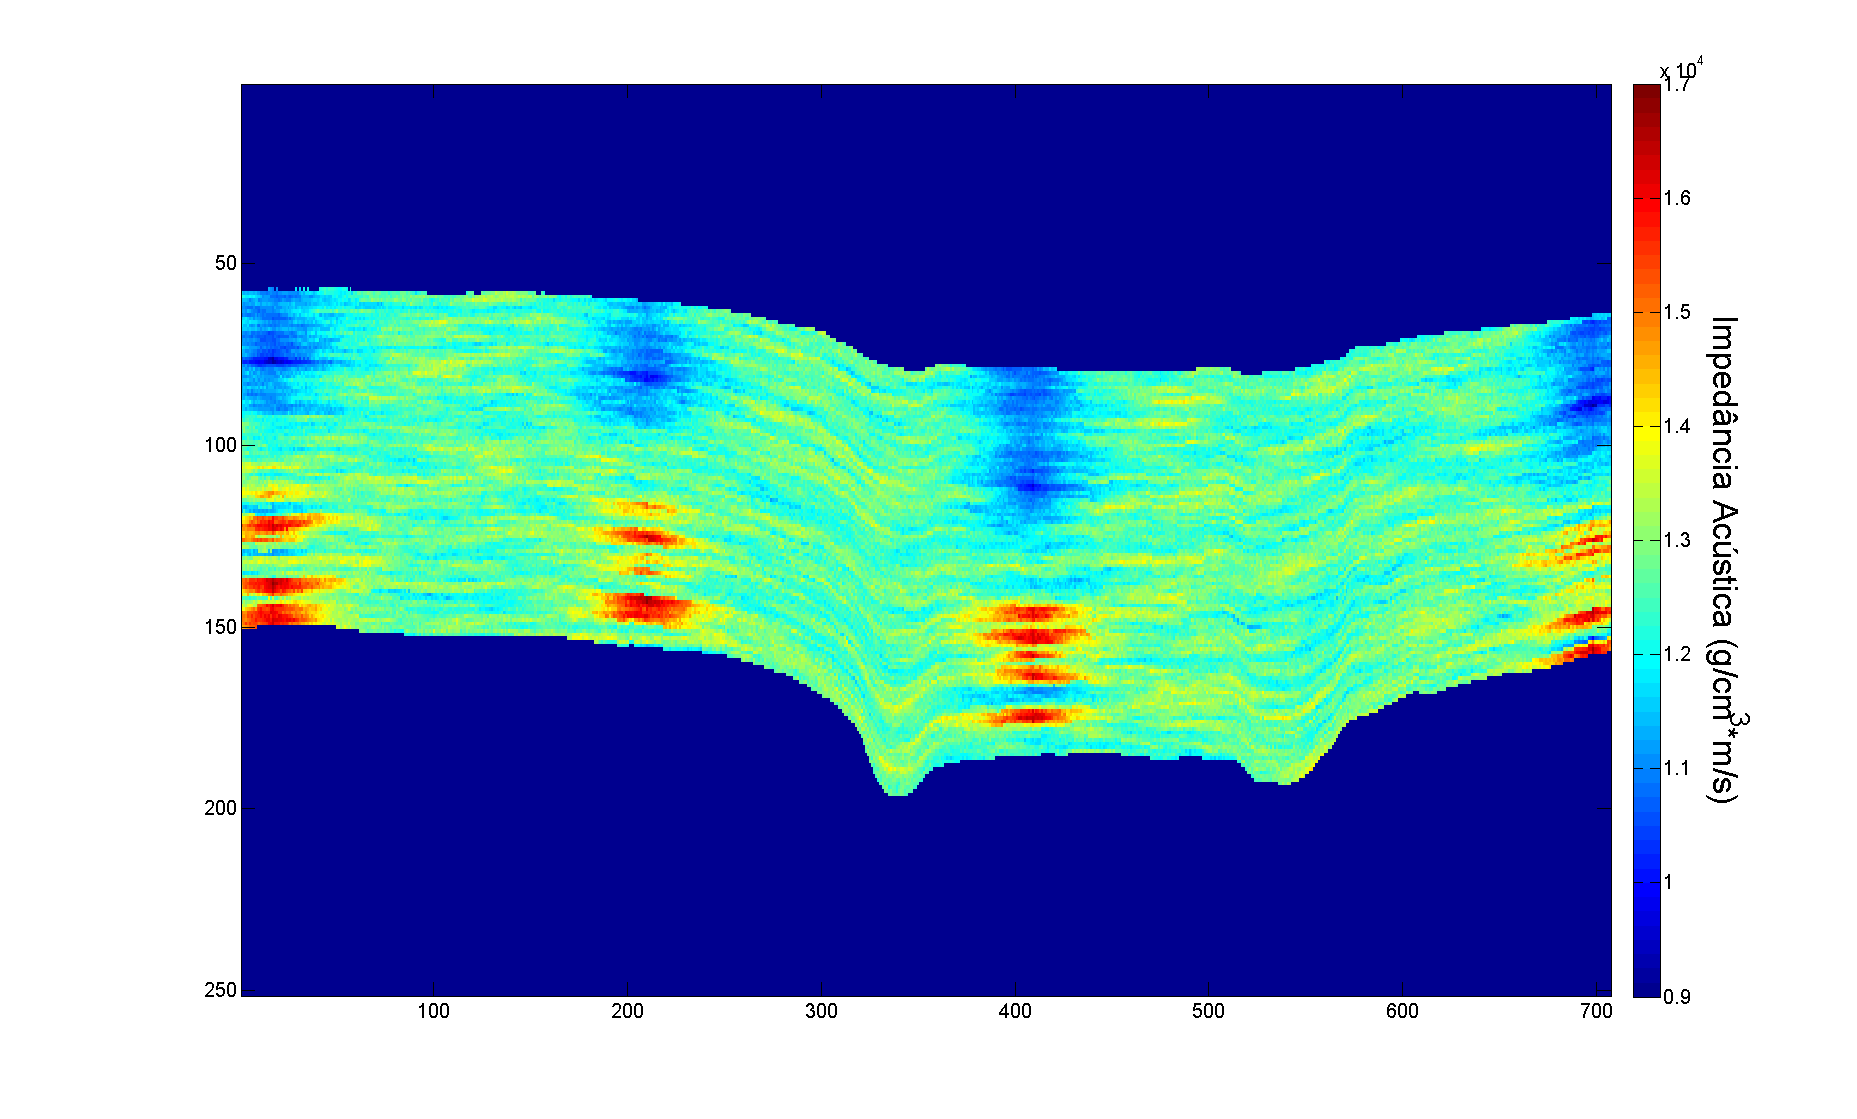
\includegraphics[width=\textwidth]{fig/dss1it-20realz}
%   \caption{Média das amostras da primeira iteração da GSI}
%   \label{fig:dssresult}
% \end{center}
% \end{figure}
% 
% \begin{figure}[htp]
% \begin{center}
%   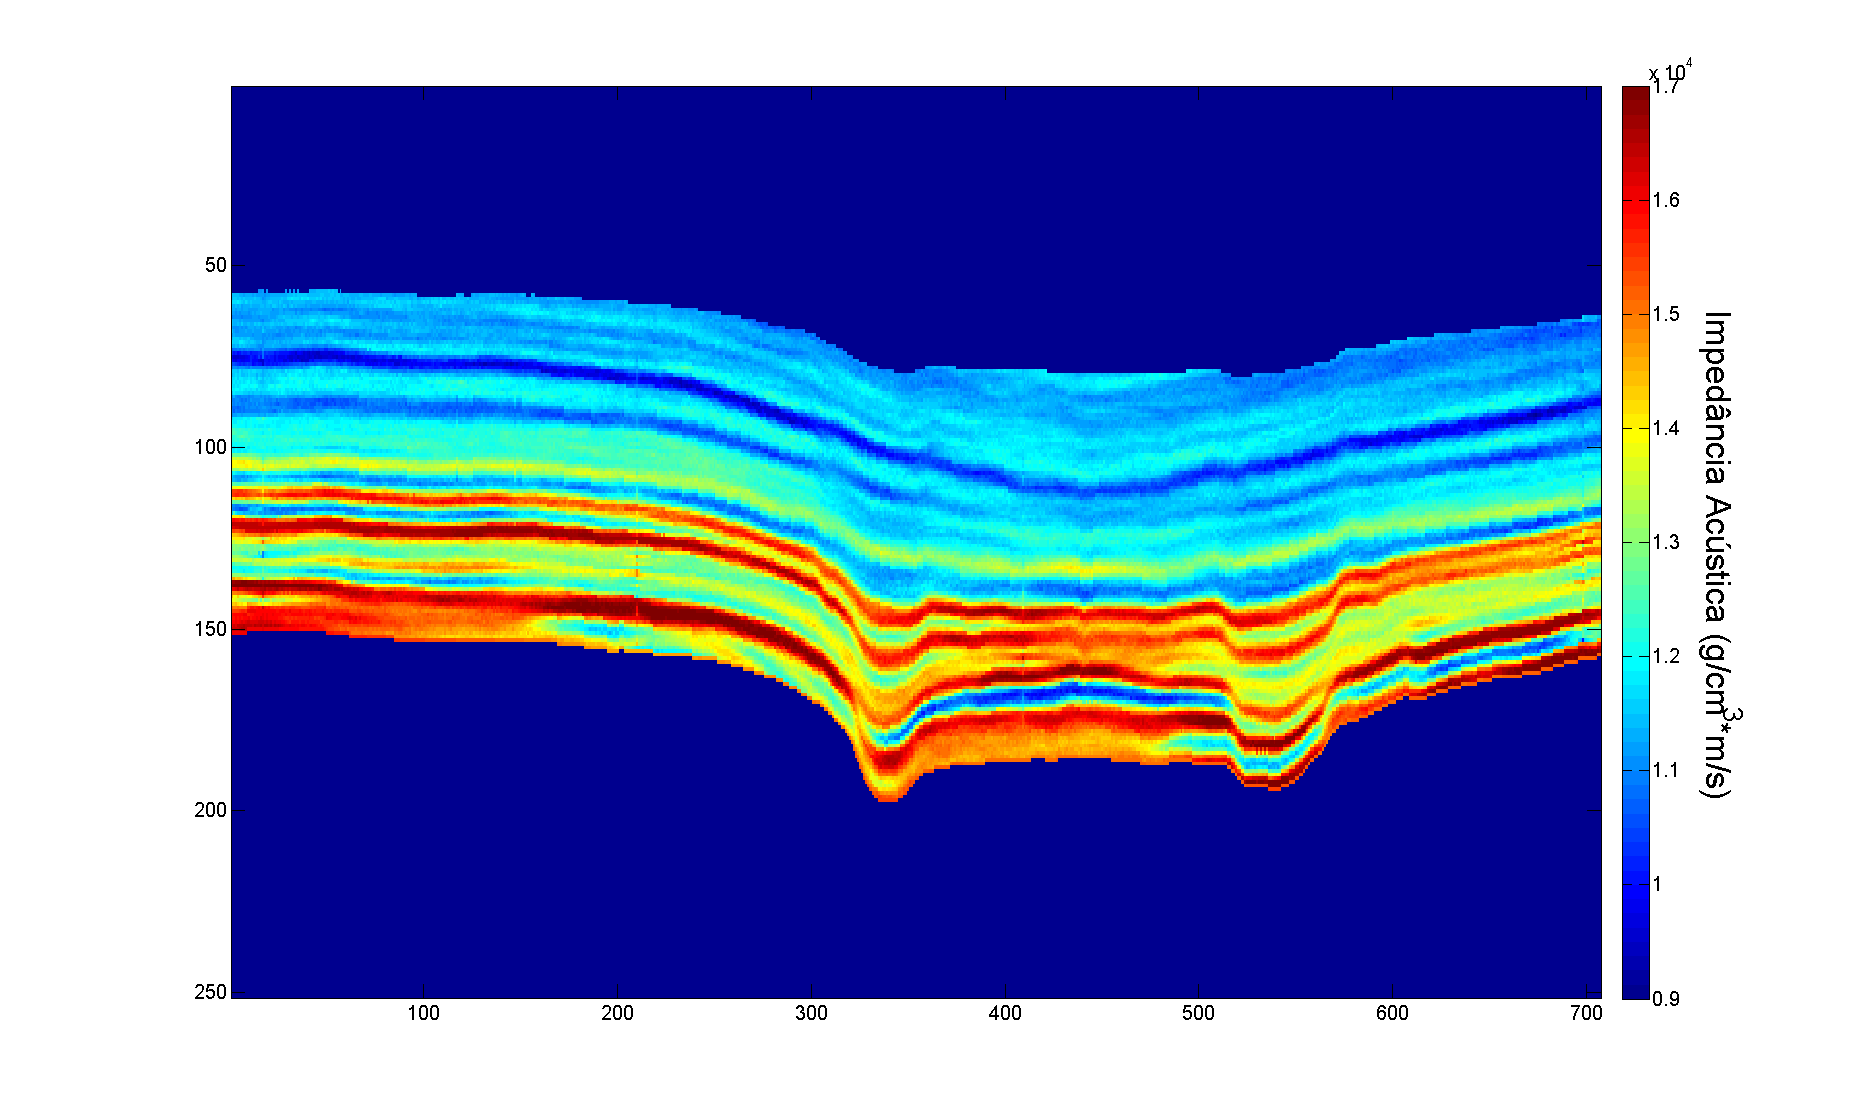
\includegraphics[width=\textwidth]{fig/mapdss1it-20realz-filt}
%   \caption{Média das amostras da SSD utilizando MAP como imagem
%   secundária}
%   \label{fig:mapDSS}
% \end{center}
% \end{figure}
% 
% 
% \begin{figure}[htp]
% \begin{center}
%   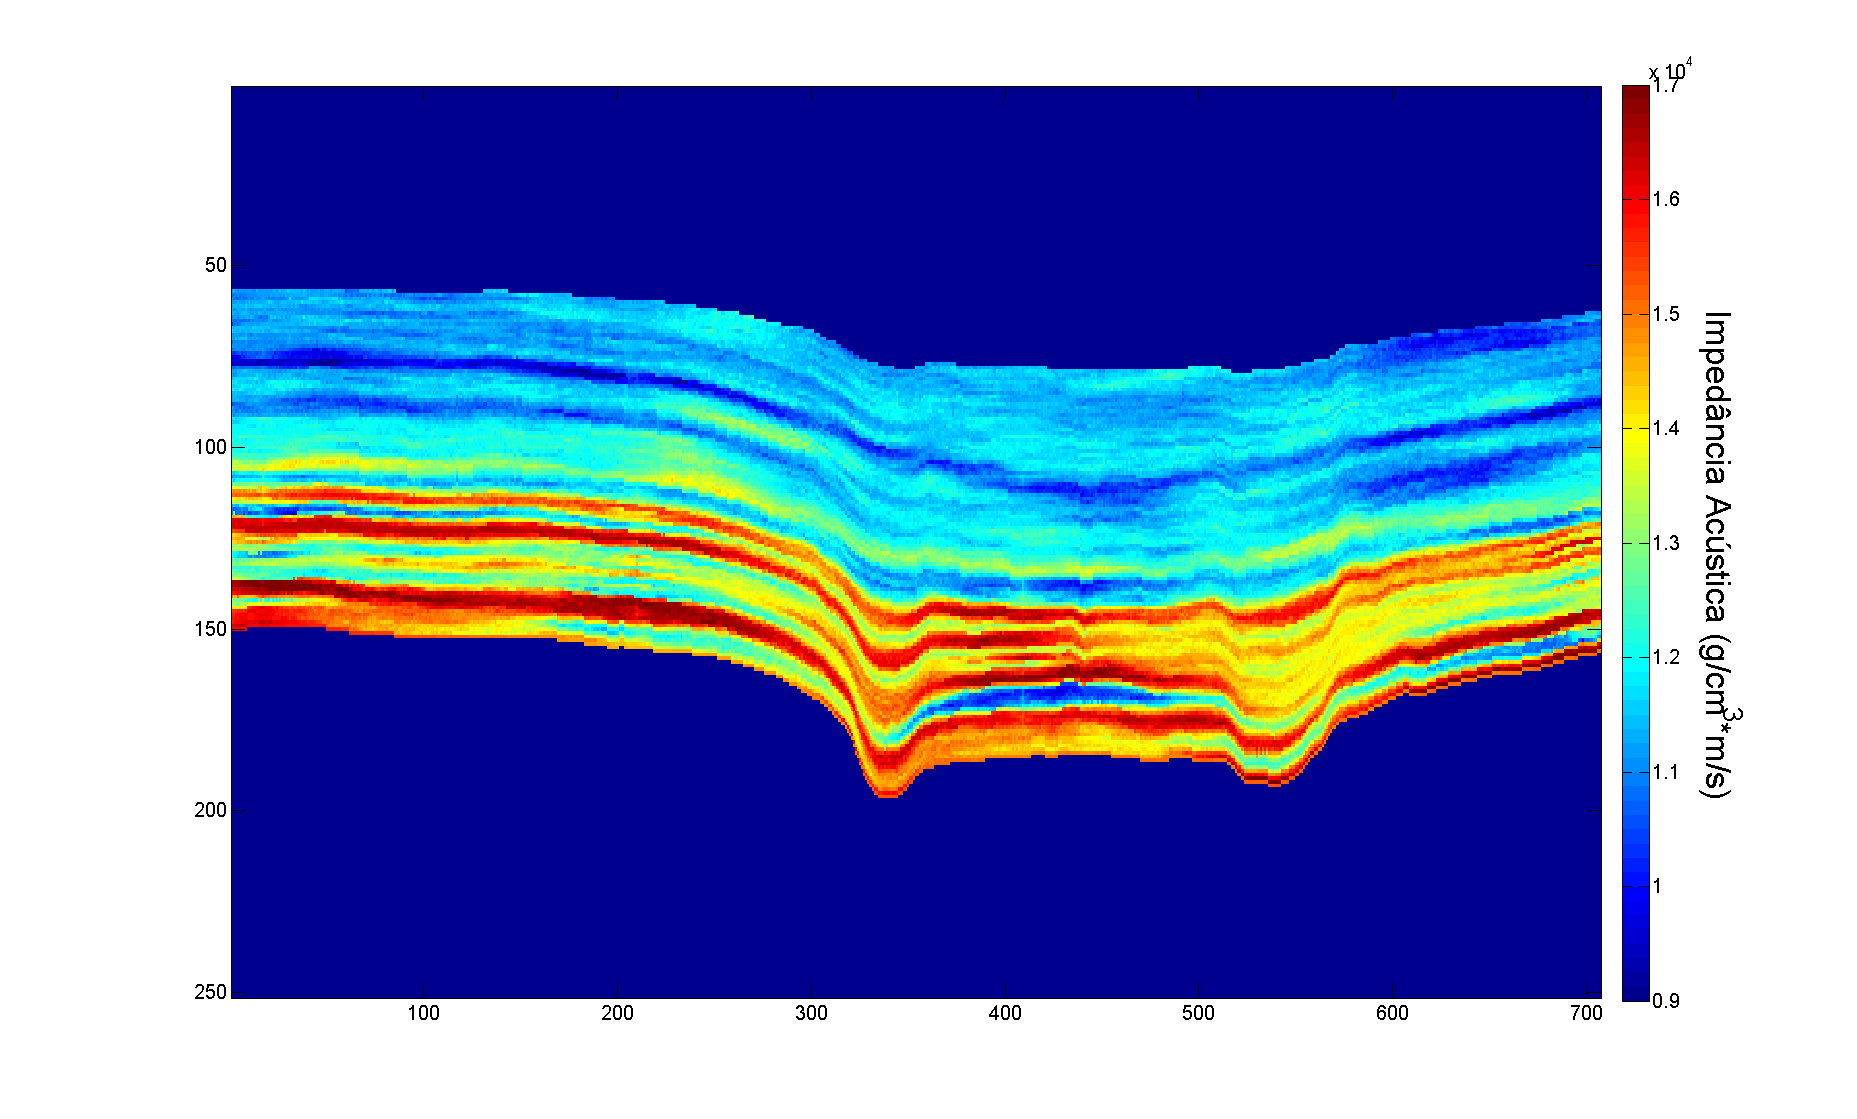
\includegraphics[width=\textwidth]{fig/dss10it-20realz}
%   \caption{Média das amostras após 10 iterações da GSI}
%   \label{fig:dss10result}
% \end{center}
% \end{figure}
% 
% A metodologia descrita na literatura para a GSI não aplica a filtragem dos dados
% para amostrar somente os resíduos, ou alta frequência. Utilizar o modelo de
% baixa frequência como informação \textit{a priori} foi identificado como uma
% regularização importante para agilizar a inversão e amostragem. Principalmente
% para a SSD, filtrar os dados resulta em uma distribuição global com menor
% variância, pois assumindo um modelo de baixa frequência são definidas médias
% locais e as amostras são geradas em torno desta média, respeitando a
% distribuição do poço filtrado. Sem a filtragem, a informação da média local não
% é utilizada, amostrando-se toda a distribuição original do poço em todos os
% pontos da região de interesse. A Figura \ref{fig:pocoFilteN} mostra a comparação
% dos histogramas dos dados filtrados e não filtrados. Portanto, utilizar o modelo
% de baixa frequência insere um viés no resultado e diminui a incerteza dada pela
% variância, mas a incerteza referente a escolha do modelo de baixa precisa ser
% levada em consideração.
% 
% 
% \begin{figure}
%         \centering
%         \begin{subfigure}[b]{0.45\textwidth}
%                 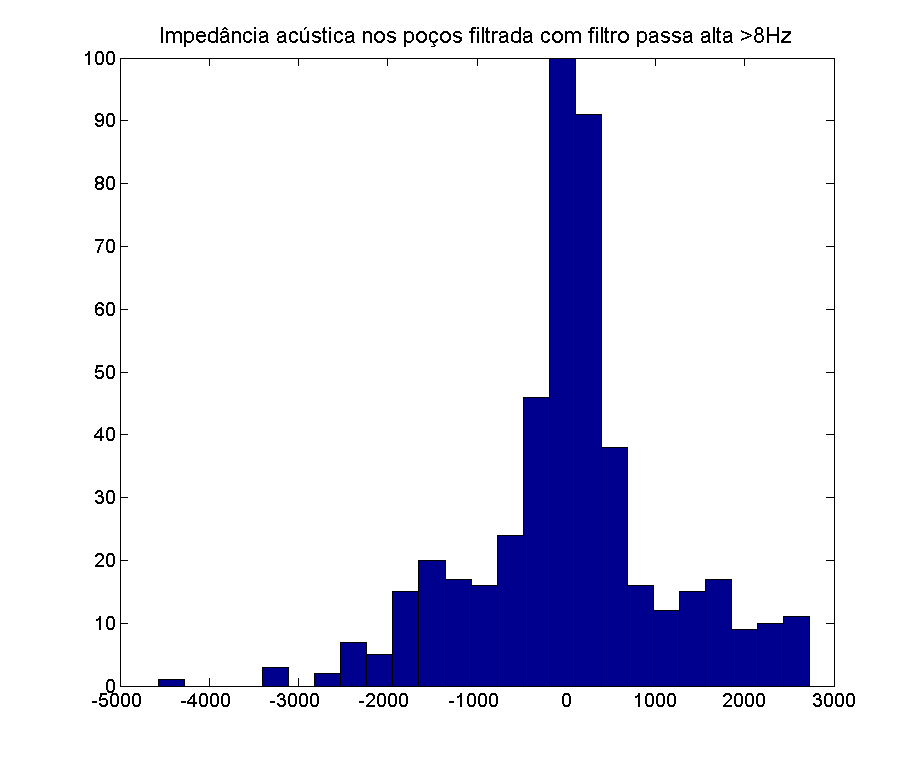
\includegraphics[width=\textwidth]{fig/IA_com_filtro}
%                 \caption{Dados filtrados}
%         \end{subfigure}%
%         \hfill
%         \begin{subfigure}[b]{0.45\textwidth}
%                 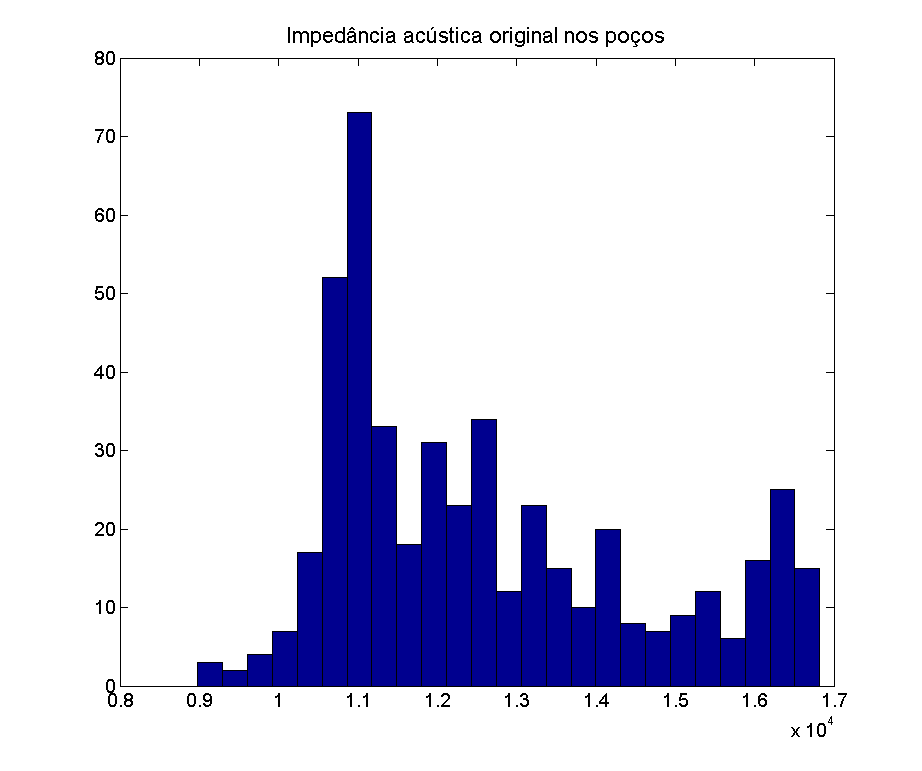
\includegraphics[width=\textwidth]{fig/IA_sem_filtro}
%                 \caption{Dados originais}
%         \end{subfigure}
%         \caption{Comparação dos dados de poços filtrados}\label{fig:pocoFilteN}
% \end{figure}
% 




\section{Proposta e Plano de Trabalho}

Os resultados preliminares apontam que é possível obter imagens de
inversão acústica em maior resolução. Entretanto, a aplicabilidade
do modelo depende da existência de conjunto de pares de imagens
de alta e baixa resolução para treinamento da rede e, consequentemente,
o limite da capacidade de inserção de altas frequências das imagens previstas
será limitada pelo faixa de altas frequências das imagens de treinamento.

contribuições esperadas para este trabalho devem alcançar ambas as
áreas de conhecimento: aprendizagem de máquina e inversão sísmica.

% A proposta para o restante do projeto é implementar a inversão elástica, que
% utiliza sísmica pré empilhada para obter as velocidades primária e secundária e
% densidade na linha de \cite{azevedo2013_avoinv} dentro da nova metodologia
% proposta. Os resultados obtidos serão comparados com os resultados da GSI em
% termos de variância e qualidade do resultado baseado na metodologia de
% \cite{coleou_qualityanomalyinv}, amplamente utilizada para avaliação dos
% resultados da inversão sísmica na indústria.
% 
% A metodologia de \cite{caers_distance_kernels_MDS} será integrada na proposta
% para possibilitar a análise da incerteza envolvida com os parâmetros e dados de
% entrada definidos pelo especialista, como o modelo de baixa, \textit{wavelets} e
% horizontes, pois a essas incertezas geológicas são apontadas como maiores
% influências na incerteza do resultado da inversão \citep[p.
% 133]{caers2011modeling}. Para tanto, será proposto um esquema de amostragem com
% Monte Carlo para selecionar os dados de entrada aleatoriamente a cada amostragem
% do resultado da inversão. Após obter várias amostras com combinações diferentes
% de dados de entrada, uma análise baseada em \textit{Multi-Dimensional Scaling}
% será aplicada para avaliar a sensibilidade ao variar cada parâmetro de entrada
% na incerteza final do resultado da inversão. Será utilizada como métrica as
% medidas de \textit{Quality-Anomaly} \citep{coleou_qualityanomalyinv}.
% 
% O caráter de originalidade do trabalho é garantido pelas contribuições para a
% área de inversão com modelagem de incerteza. A primeira contribuição diminui o
% tempo de execução por eliminar a necessidade de um método iterativo para
% realizar a inversão geoestatística, ao mesmo tempo modelando a continuidade
% lateral. A segunda contribuição será modelar as incertezas presentes nos dados
% de entrada (\textit{wavelets}, horizontes, modelos de baixa, variogramas,
% etc\ldots) após a integração da metodologia de
% \cite{caers_distance_kernels_MDS}.
% 
% A Figura \ref{fig:gantt} mostra o cronograma mensal das atividades a serem
% desenvolvidas durante o período de 12 meses do estágio de doutorado sanduíche a
% ser realizado no Centro de Recursos Naturais e Ambiente (CERENA) do Instituto
% Superior Técnico (IST) ligado a Universidade de Lisboa sob orientação do Dr.
% Amilcar Soares. Também estão planejados os meses após o retorno para finalização
% da tese e defesa.
% 
% 
% \begin{figure}[htp]
% \begin{center}
%   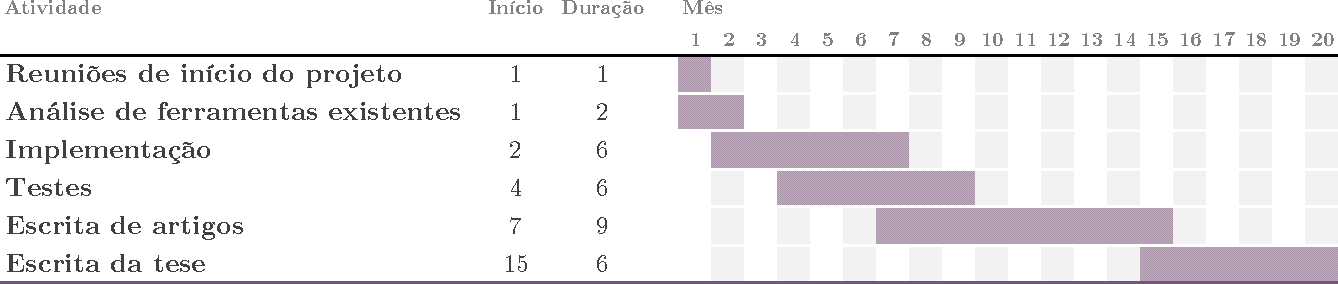
\includegraphics[width=\textwidth]{fig/gantt_EQD}
%   \caption{Cronograma mensal do projeto a partir de jul/2014}
%   \label{fig:gantt}
% \end{center}
% \end{figure}
% 
% Dentre os periódicos que apresentam trabalhos relacionados com esta área, se
% destacam os seguintes com suas classificações no Qualis para Ciências da
% Computação:
% 
% \begin{itemize}
%   \setlength{\itemsep}{0pt}
%   \setlength{\parskip}{0pt}
%   \item IEEE Trans. on Geoscience and Remote Sensing
%   \item ISSN: 0196-2892 - IEEE - Qualis A1
% \end{itemize}
% 
% \begin{itemize}
%   \setlength{\itemsep}{0pt}
%   \setlength{\parskip}{0pt}
%   \item Journal of Computational Physics
%   \item ISSN: 0021-9991 - Elsevier - Qualis A1
% \end{itemize}
% 
% \begin{itemize}
%   \setlength{\itemsep}{0pt}
%   \setlength{\parskip}{0pt}
%   \item Computers \& Geosciences
%   \item ISSN: 0098-3004 - Elsevier - Qualis A2
% \end{itemize}
% 
% 
% \begin{itemize}
%   \setlength{\itemsep}{0pt}
%   \setlength{\parskip}{0pt}
%   \item Computational Geosciences
%   \item ISSN: 1420-0597 - Springer - Qualis B1
% \end{itemize}
% 
% 
% \begin{itemize}
%   \setlength{\itemsep}{0pt}
%   \setlength{\parskip}{0pt}
%   \item Geophysics
%   \item ISSN: 0016-8033 - Society of Exploration Geophysicists - Qualis A2 Interdisciplinar
% \end{itemize}
% 
% 
% \begin{itemize}
%   \setlength{\itemsep}{0pt}
%   \setlength{\parskip}{0pt}
%   \item Mathematical Geosciences
%   \item ISSN: 1874-8961 - Springer - Qualis A2 Interdisciplinar
% \end{itemize}
% 
% 
% A colaboração com o grupo de pesquisas do Prof. Amilcar Soares é justificada
% pois o autor é a uma das principais referências na literatura sobre Simulação
% Sequencial Direta e inversão Geoestatística
% \citep{azevedo2013_avoinv,amilcarInversao,2001amilcarDSS}. A pesquisa nos dois
% primeiros anos do projeto de Doutorado foi feita sob orientação do Prof. Mauro
% Roisenberg, coautor de referências relevantes para inversão Bayesiana
% \citep{leandro_SEG,leandroGRSL}. Desta forma, espera-se cumprir a proposta de
% integração sob orientação de especialistas em ambos os métodos. A proposta
% também faz parte de um Termo de Cooperação Petrobras/UFSC/FEESC.
% 
% 
